\chapter{Übungen}

\section{Übung 1 – Analoge Signale}

Dieses Übungsblatt behandelt die grundlegenden Eigenschaften analoger Signale:
den Signalverlauf, die Unterscheidung in Energie- und Leistungssignale
(Abschnitte~\ref{sec:norm-energie-leistung} und~\ref{sec:leistung}), die
Symmetrieeigenschaften (Abschnitt~\ref{sec:symmetrie-signale}), Periodizität
(Abschnitt~\ref{sec:periodische-signale}), den Mittelwert
(Abschnitt~\ref{sec:mittelwert}) sowie komplexwertige Signale
(Abschnitt~\ref{sec:komplexwertige-signale}). Für die Rechteck- und
Sprungfunktion wird durchgehend die Skript-Definition aus
Abschnitt~\ref{sec:elementare-analoge-signale} verwendet:
$\operatorname{rect}(u) = 1$ für $0 \leq u < 1$ (sonst $0$) und
$\epsilon(t) = 1$ für $t \geq 0$ (sonst $0$).

% ================================================================
\subsection*{Vorrechenaufgabe 1 – Signalanalyse}
% ================================================================

Für die folgenden Signale ist der Signalverlauf zu skizzieren und zu prüfen, ob
ein Energie- oder ein Leistungssignal vorliegt. Zur Klassifikation dienen
Energie und Leistung (Abschnitte~\ref{sec:norm-energie-leistung}
und~\ref{sec:leistung}):

$$
E_x = \int_{-\infty}^{\infty} |x(t)|^2\,\mathrm{d}t,
\qquad
P_x = \lim_{T_0 \to \infty} \frac{1}{2T_0} \int_{-T_0}^{T_0} |x(t)|^2\,\mathrm{d}t.
$$

Ein \emph{Energiesignal} besitzt $0 < E_x < \infty$ (und $P_x = 0$), ein
\emph{Leistungssignal} $0 < P_x < \infty$ (und $E_x = \infty$).

% ---- a) --------------------------------------------------------
\subsubsection*{a) Rechteckimpuls}

\begin{beispiel}[Verschobener Rechteckimpuls]

\textbf{Gegeben:} $x(t) = \operatorname{rect}\!\left(\dfrac{t + T}{2T}\right)$
mit $T > 0$ (Abschnitt~\ref{sec:elementare-analoge-signale}).

\textbf{Gesucht:} Signalverlauf; Energie- oder Leistungssignal?

\textbf{Formel:} Rechteck-Definition sowie Energie
(Abschnitt~\ref{sec:norm-energie-leistung}).

\textbf{Rechnung:}

Das Argument liegt im Trägerbereich, wenn
$0 \leq \dfrac{t+T}{2T} < 1$, also $-T \leq t < T$. Dort ist $x(t) = 1$, sonst
$0$. Es handelt sich um einen Rechteckimpuls der Höhe $1$ und Breite $2T$,
zentriert um $t = 0$.

$$
E_x = \int_{-T}^{T} 1^2\,\mathrm{d}t = 2T < \infty.
$$

\begin{center}
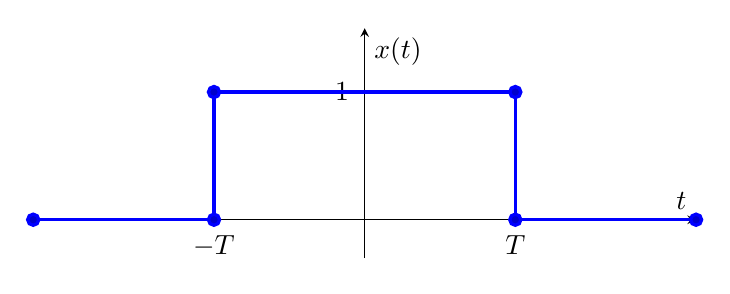
\begin{tikzpicture}
\begin{axis}[
  width=10cm, height=4.5cm,
  xmin=-2.2, xmax=2.2, ymin=-0.3, ymax=1.5,
  axis lines=center,
  xlabel={$t$}, ylabel={$x(t)$},
  xtick={-1,1}, xticklabels={$-T$,$T$},
  ytick={1}, yticklabels={$1$},
  every axis plot/.append style={very thick, blue},
]
\addplot coordinates {(-2.2,0) (-1,0) (-1,1) (1,1) (1,0) (2.2,0)};
\end{axis}
\end{tikzpicture}
\end{center}

\textbf{Lösung:}

$$
\boxed{\;E_x = 2T < \infty \;\Rightarrow\; \text{Energiesignal.}\;}
$$

\end{beispiel}

% ---- b) --------------------------------------------------------
\subsubsection*{b) Abklingende Exponentialfunktion}

\begin{beispiel}[Einseitig abklingende Exponentialfunktion]

\textbf{Gegeben:} $x(t) = 2\,e^{-t/T}\,\epsilon(t)$ mit $T > 0$.

\textbf{Gesucht:} Signalverlauf; Energie- oder Leistungssignal?

\textbf{Formel:} Energie (Abschnitt~\ref{sec:norm-energie-leistung}).

\textbf{Rechnung:}

Für $t < 0$ ist $x(t) = 0$, für $t \geq 0$ fällt $x(t)$ von $x(0) = 2$
monoton gegen $0$ ab.

$$
E_x = \int_0^{\infty} \left(2\,e^{-t/T}\right)^2 \mathrm{d}t
    = 4 \int_0^{\infty} e^{-2t/T}\,\mathrm{d}t
    = 4 \cdot \frac{T}{2} = 2T < \infty.
$$

\begin{center}
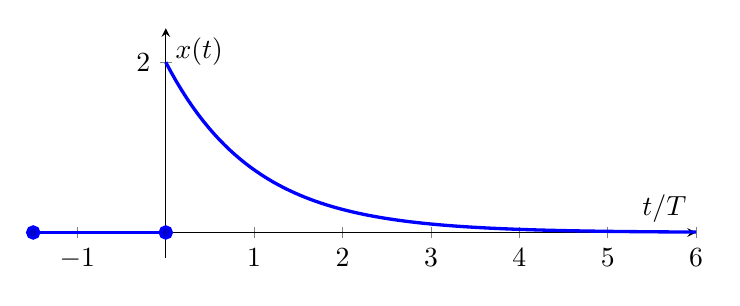
\begin{tikzpicture}
\begin{axis}[
  width=10cm, height=4.5cm,
  xmin=-1.5, xmax=6, ymin=-0.3, ymax=2.4,
  axis lines=center,
  xlabel={$t/T$}, ylabel={$x(t)$},
  ytick={2}, yticklabels={$2$},
  samples=100,
  every axis plot/.append style={very thick, blue},
]
\addplot coordinates {(-1.5,0) (0,0)};
\addplot[domain=0:6] {2*exp(-x)};
\end{axis}
\end{tikzpicture}
\end{center}

\textbf{Lösung:}

$$
\boxed{\;E_x = 2T < \infty \;\Rightarrow\; \text{Energiesignal.}\;}
$$

\end{beispiel}

% ---- c) --------------------------------------------------------
\subsubsection*{c) Aufladende Exponentialfunktion}

\begin{beispiel}[Einseitig aufladende Exponentialfunktion]

\textbf{Gegeben:} $x(t) = 4\left(1 - e^{-2t/T}\right)\epsilon(t)$ mit $T > 0$.

\textbf{Gesucht:} Signalverlauf; Energie- oder Leistungssignal?

\textbf{Formel:} Energie und Leistung (Abschnitte~\ref{sec:norm-energie-leistung}
und~\ref{sec:leistung}).

\textbf{Rechnung:}

Für $t \geq 0$ steigt $x(t)$ von $0$ monoton gegen den Grenzwert $4$. Da $x(t)$
für $t \to \infty$ konstant $4$ bleibt, ist die Energie unbeschränkt
($E_x = \infty$). Die Leistung ist dagegen endlich:

$$
P_x = \lim_{T_0 \to \infty} \frac{1}{2T_0} \int_0^{T_0}
      16\left(1 - e^{-2t/T}\right)^2 \mathrm{d}t
    = \lim_{T_0 \to \infty} \frac{16\,T_0 - 12\,T}{2T_0}
    = \frac{16}{2} = 8.
$$

\begin{center}
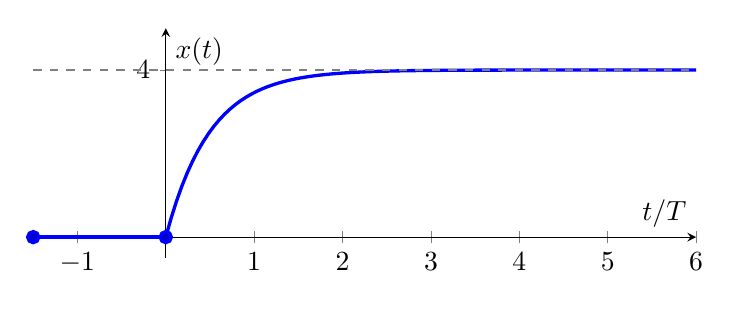
\begin{tikzpicture}
\begin{axis}[
  width=10cm, height=4.5cm,
  xmin=-1.5, xmax=6, ymin=-0.5, ymax=5,
  axis lines=center,
  xlabel={$t/T$}, ylabel={$x(t)$},
  ytick={4}, yticklabels={$4$},
  samples=100,
  every axis plot/.append style={very thick, blue},
]
\addplot coordinates {(-1.5,0) (0,0)};
\addplot[domain=0:6] {4*(1-exp(-2*x))};
\draw[dashed, gray] (axis cs:-1.5,4) -- (axis cs:6,4);
\end{axis}
\end{tikzpicture}
\end{center}

\textbf{Lösung:}

$$
\boxed{\;E_x = \infty,\quad P_x = 8 \;\Rightarrow\; \text{Leistungssignal.}\;}
$$

\end{beispiel}

% ---- d) --------------------------------------------------------
\subsubsection*{d) Sinusförmiges Signal}

\begin{beispiel}[Sinusförmiges Signal mit Symmetrie, Mittelwert und Leistung]

\textbf{Gegeben:}
$x(t) = 2\sin\!\left(\dfrac{2\pi}{1\,\mathrm{s}}\,t\right)
= 2\sin\!\left(2\pi\dfrac{t}{T}\right) = 2\sin(\omega t) = 2\sin(2\pi f t)$.

\textbf{Gesucht:} Signalverlauf, Kenngrößen $T,\, f,\, \omega$,
Symmetrieeigenschaft, Mittelwert und Leistung.

\textbf{Formel:} Periodendauer, Symmetrie, Mittelwert und Leistung
(Abschnitte~\ref{sec:periodische-signale}, \ref{sec:symmetrie-signale},
\ref{sec:mittelwert-periodisch} und~\ref{sec:leistung}).

\textbf{Rechnung:}

Koeffizientenvergleich liefert $\omega = \dfrac{2\pi}{1\,\mathrm{s}}$, also

$$
\omega = 2\pi\,\mathrm{s}^{-1}, \qquad
f = \frac{\omega}{2\pi} = 1\,\mathrm{Hz}, \qquad
T = \frac{1}{f} = 1\,\mathrm{s}.
$$

Wegen $\sin(-\omega t) = -\sin(\omega t)$ ist $x(t)$ \emph{ungerade}. Der
Mittelwert über eine Periode verschwindet, und die Leistung eines
Sinussignals der Amplitude $A$ beträgt $A^2/2$:

$$
\bar{x} = \frac{1}{T}\int_0^T 2\sin(\omega t)\,\mathrm{d}t = 0,
\qquad
P_x = \frac{1}{T}\int_0^T 4\sin^2(\omega t)\,\mathrm{d}t
    = \frac{A^2}{2} = \frac{2^2}{2} = 2.
$$

\begin{center}
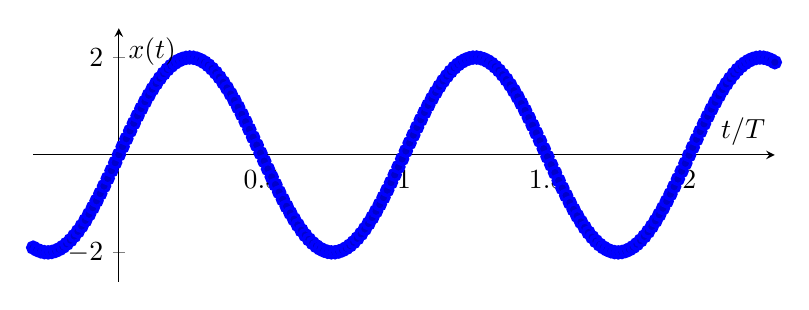
\begin{tikzpicture}
\begin{axis}[
  width=11cm, height=4.8cm,
  xmin=-0.3, xmax=2.3, ymin=-2.6, ymax=2.6,
  axis lines=center,
  xlabel={$t/T$}, ylabel={$x(t)$},
  ytick={-2,2}, yticklabels={$-2$,$2$},
  samples=200, domain=-0.3:2.3,
  every axis plot/.append style={very thick, blue},
]
\addplot {2*sin(360*x)};
\end{axis}
\end{tikzpicture}
\end{center}

\textbf{Lösung:}

$$
\boxed{\;T = 1\,\mathrm{s},\;\; f = 1\,\mathrm{Hz},\;\;
\omega = 2\pi\,\mathrm{s}^{-1};\quad
\text{ungerade},\;\; \bar{x} = 0,\;\; P_x = 2 \;\Rightarrow\;
\text{Leistungssignal.}\;}
$$

\end{beispiel}

% ---- e) --------------------------------------------------------
\subsubsection*{e) Komplexwertiges Exponentialsignal}

\begin{beispiel}[Zusammenhang zwischen Betrag, Phase und Real- bzw. Imaginärteil]

\textbf{Gegeben:} Komplexe Zahl $x = A\cdot e^{j\varphi}$ sowie das
komplexwertige Signal $\underline{x}(t) = e^{j\pi t}$
(Abschnitt~\ref{sec:komplexe-exponentialsignale}).

\textbf{Gesucht:} Grafischer und rechnerischer Zusammenhang zwischen
$\sin\varphi$, $\cos\varphi$ und Real- bzw.\ Imaginärteil; anschließend
$\operatorname{Re}\{\underline{x}(t)\}$, $\operatorname{Im}\{\underline{x}(t)\}$,
$T$, $f$, Mittelwert und Leistung von $\underline{x}(t)$.

\textbf{Formel} (Eulersche Formel, Abschnitt~\ref{sec:komplexe-exponentialsignale}):

$$
A\, e^{j\varphi} = A\cos\varphi + j\,A\sin\varphi,
\qquad
\operatorname{Re}\{x\} = A\cos\varphi, \quad
\operatorname{Im}\{x\} = A\sin\varphi.
$$

\textbf{Rechnung:}

Grafisch entspricht $x = A\,e^{j\varphi}$ einem Zeiger der Länge $A$ unter dem
Winkel $\varphi$ in der komplexen Ebene. Die Projektion auf die reelle Achse
liefert $A\cos\varphi$, die Projektion auf die imaginäre Achse $A\sin\varphi$:

\begin{center}
\begin{tikzpicture}[scale=2.2]
  \draw[->] (-1.3,0) -- (1.4,0) node[right] {$\operatorname{Re}$};
  \draw[->] (0,-0.4) -- (0,1.3) node[above] {$\operatorname{Im}$};
  \draw[gray, dashed] (0,0) circle (1);
  \def\ang{55}
  \draw[very thick, blue, ->] (0,0) -- (\ang:1) node[midway, above left] {$A$};
  \draw[dashed] (\ang:1) -- ({cos(\ang)},0);
  \draw[dashed] (\ang:1) -- (0,{sin(\ang)});
  \draw[red, thick] (0,0) -- ({cos(\ang)},0)
        node[midway, below] {$A\cos\varphi$};
  \draw[red, thick] (0,{sin(\ang)}) -- (\ang:1)
        node[midway, above] {$A\sin\varphi$};
  \draw (0.3,0) arc (0:\ang:0.3);
  \node at (28:0.42) {$\varphi$};
\end{tikzpicture}
\end{center}

Für $\underline{x}(t) = e^{j\pi t}$ gilt $A = 1$ und $\varphi(t) = \pi t$, also

$$
\operatorname{Re}\{\underline{x}(t)\} = \cos(\pi t), \qquad
\operatorname{Im}\{\underline{x}(t)\} = \sin(\pi t).
$$

Aus $\omega = \pi\,\mathrm{s}^{-1}$ folgt

$$
f = \frac{\omega}{2\pi} = \frac{1}{2}\,\mathrm{Hz}, \qquad
T = \frac{1}{f} = 2\,\mathrm{s}.
$$

Wegen $|\underline{x}(t)| = 1$ und der vollständigen Umdrehung pro Periode:

$$
\bar{\underline{x}} = \frac{1}{T}\int_0^T e^{j\pi t}\,\mathrm{d}t = 0,
\qquad
P_{\underline{x}} = \frac{1}{T}\int_0^T |e^{j\pi t}|^2\,\mathrm{d}t = 1.
$$

\begin{center}
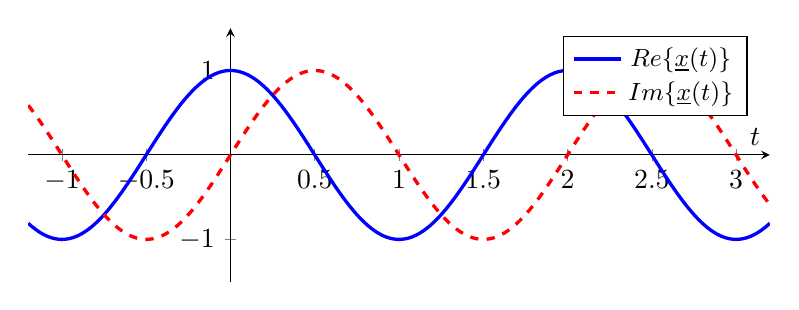
\begin{tikzpicture}
\begin{axis}[
  width=11cm, height=4.8cm,
  xmin=-1.2, xmax=3.2, ymin=-1.5, ymax=1.5,
  axis lines=center,
  xlabel={$t$}, ylabel={},
  ytick={-1,1}, yticklabels={$-1$,$1$},
  samples=200, domain=-1.2:3.2,
  legend pos=north east, legend style={font=\small},
  every axis plot/.append style={very thick},
]
\addplot[blue] {cos(180*x)}; \addlegendentry{$\operatorname{Re}\{\underline{x}(t)\}$}
\addplot[red, dashed] {sin(180*x)}; \addlegendentry{$\operatorname{Im}\{\underline{x}(t)\}$}
\end{axis}
\end{tikzpicture}
\end{center}

\textbf{Lösung:}

$$
\boxed{\;\operatorname{Re}\{\underline{x}\} = \cos(\pi t),\;\;
\operatorname{Im}\{\underline{x}\} = \sin(\pi t);\;\;
T = 2\,\mathrm{s},\;\; f = \tfrac12\,\mathrm{Hz},\;\;
\bar{\underline{x}} = 0,\;\; P_{\underline{x}} = 1.\;}
$$

$\underline{x}(t)$ ist ein Leistungssignal mit konstantem Betrag $1$.

\end{beispiel}

% ================================================================
\subsection*{Aufgabe 1.1 – Einheitssprung}
% ================================================================

Die folgenden Signale sind unter Beachtung aller charakteristischen Werte als
Funktion der Zeit zu zeichnen; abschließend erfolgt die Klassifikation in
Energie- oder Leistungssignale.

\subsubsection*{a) $x(t) = 2 - 2\epsilon(t)$}

\begin{beispiel}[Absteigende Sprungfunktion]

\textbf{Gegeben:} $x(t) = 2 - 2\epsilon(t)$
(Abschnitt~\ref{sec:elementare-analoge-signale}).

\textbf{Gesucht:} Signalverlauf; Energie- oder Leistungssignal?

\textbf{Formel:} Sprung-Definition sowie Leistung
(Abschnitt~\ref{sec:leistung}).

\textbf{Rechnung:} Für $t < 0$ ist $\epsilon(t) = 0$, also $x = 2$; für
$t \geq 0$ ist $x = 2 - 2 = 0$. Da $x(t) = 2$ für alle $t < 0$ gilt, ist
$E_x = \infty$; die Leistung ist

$$
P_x = \lim_{T_0 \to \infty} \frac{1}{2T_0}\int_{-T_0}^{0} 2^2\,\mathrm{d}t
    = \lim_{T_0 \to \infty} \frac{4\,T_0}{2T_0} = 2.
$$

\begin{center}
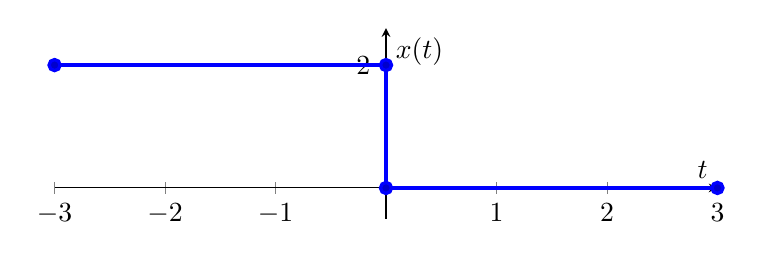
\begin{tikzpicture}
\begin{axis}[
  width=10cm, height=4cm,
  xmin=-3, xmax=3, ymin=-0.5, ymax=2.6,
  axis lines=center, xlabel={$t$}, ylabel={$x(t)$},
  ytick={2}, yticklabels={$2$},
  every axis plot/.append style={very thick, blue},
]
\addplot coordinates {(-3,2) (0,2) (0,0) (3,0)};
\end{axis}
\end{tikzpicture}
\end{center}

\textbf{Lösung:} $\boxed{\;P_x = 2 \Rightarrow \text{Leistungssignal.}\;}$

\end{beispiel}

\subsubsection*{b) $x(t) = \epsilon(t) - \epsilon(t-1\,\mathrm{ms}) + \epsilon(t-2\,\mathrm{ms}) - \epsilon(t-3\,\mathrm{ms})$}

\begin{beispiel}[Zwei Rechteckimpulse aus Sprungfunktionen]

\textbf{Gegeben:} $x(t) = \epsilon(t) - \epsilon(t-1\,\mathrm{ms})
+ \epsilon(t-2\,\mathrm{ms}) - \epsilon(t-3\,\mathrm{ms})$.

\textbf{Gesucht:} Signalverlauf; Energie- oder Leistungssignal?

\textbf{Rechnung:} Abschnittsweise Auswertung ergibt zwei Rechteckimpulse der
Höhe $1$: auf $[0,1\,\mathrm{ms})$ und auf $[2\,\mathrm{ms},3\,\mathrm{ms})$.
Endliche Dauer, also Energiesignal mit

$$
E_x = 1^2\cdot 1\,\mathrm{ms} + 1^2\cdot 1\,\mathrm{ms}
    = 2\,\mathrm{ms}.
$$

\begin{center}
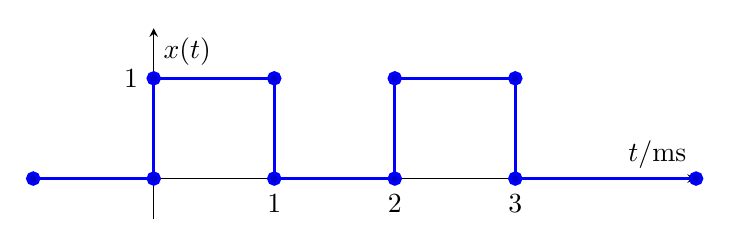
\begin{tikzpicture}
\begin{axis}[
  width=10cm, height=4cm,
  xmin=-1, xmax=4.5, ymin=-0.4, ymax=1.5,
  axis lines=center, xlabel={$t/\mathrm{ms}$}, ylabel={$x(t)$},
  xtick={1,2,3}, ytick={1}, yticklabels={$1$},
  every axis plot/.append style={very thick, blue},
]
\addplot coordinates {(-1,0) (0,0) (0,1) (1,1) (1,0) (2,0) (2,1) (3,1) (3,0) (4.5,0)};
\end{axis}
\end{tikzpicture}
\end{center}

\textbf{Lösung:} $\boxed{\;E_x = 2\,\mathrm{ms} \Rightarrow \text{Energiesignal.}\;}$

\end{beispiel}

\subsubsection*{c) $x(t) = \operatorname{rect}\!\left(\dfrac{t-2\,\mathrm{ms}}{4\,\mathrm{ms}}\right)$}

\begin{beispiel}[Rechteckimpuls über die Rechteckfunktion]

\textbf{Gegeben:} $x(t) = \operatorname{rect}\!\left(\dfrac{t-2\,\mathrm{ms}}{4\,\mathrm{ms}}\right)$.

\textbf{Gesucht:} Signalverlauf; Energie- oder Leistungssignal?

\textbf{Rechnung:} Trägerbedingung $0 \leq \dfrac{t-2\,\mathrm{ms}}{4\,\mathrm{ms}} < 1$
liefert $2\,\mathrm{ms} \leq t < 6\,\mathrm{ms}$; dort $x = 1$. Rechteck der
Höhe $1$ und Breite $4\,\mathrm{ms}$.

$$
E_x = 1^2 \cdot 4\,\mathrm{ms} = 4\,\mathrm{ms}.
$$

\begin{center}
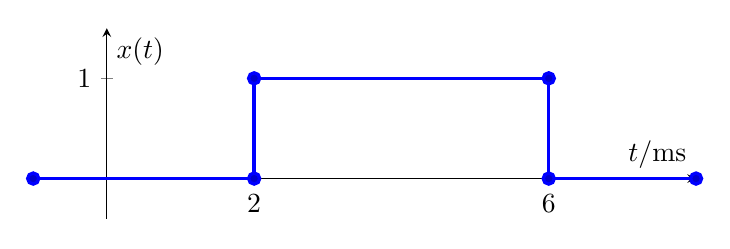
\begin{tikzpicture}
\begin{axis}[
  width=10cm, height=4cm,
  xmin=-1, xmax=8, ymin=-0.4, ymax=1.5,
  axis lines=center, xlabel={$t/\mathrm{ms}$}, ylabel={$x(t)$},
  xtick={2,6}, ytick={1}, yticklabels={$1$},
  every axis plot/.append style={very thick, blue},
]
\addplot coordinates {(-1,0) (2,0) (2,1) (6,1) (6,0) (8,0)};
\end{axis}
\end{tikzpicture}
\end{center}

\textbf{Lösung:} $\boxed{\;E_x = 4\,\mathrm{ms} \Rightarrow \text{Energiesignal.}\;}$

\end{beispiel}

\subsubsection*{d) $x(t) = \pi\left[\epsilon(t-T) - \epsilon(t-3T)\right]$}

\begin{beispiel}[Skalierter Rechteckimpuls aus Sprungfunktionen]

\textbf{Gegeben:} $x(t) = \pi\left[\epsilon(t-T) - \epsilon(t-3T)\right]$,
$T > 0$.

\textbf{Gesucht:} Signalverlauf; Energie- oder Leistungssignal?

\textbf{Rechnung:} Rechteckimpuls der Höhe $\pi$ auf $[T, 3T)$, Breite $2T$.

$$
E_x = \pi^2 \cdot 2T = 2\pi^2 T.
$$

\begin{center}
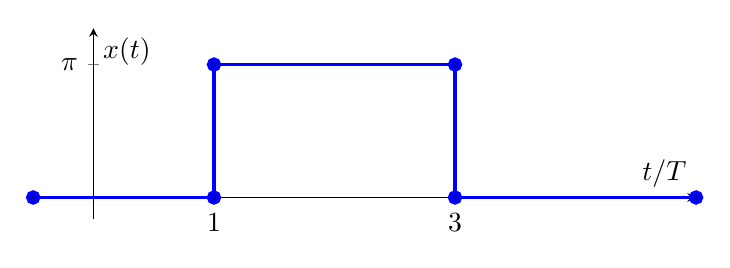
\begin{tikzpicture}
\begin{axis}[
  width=10cm, height=4cm,
  xmin=-0.5, xmax=5, ymin=-0.5, ymax=4,
  axis lines=center, xlabel={$t/T$}, ylabel={$x(t)$},
  xtick={1,3}, ytick={3.1416}, yticklabels={$\pi$},
  every axis plot/.append style={very thick, blue},
]
\addplot coordinates {(-0.5,0) (1,0) (1,3.1416) (3,3.1416) (3,0) (5,0)};
\end{axis}
\end{tikzpicture}
\end{center}

\textbf{Lösung:} $\boxed{\;E_x = 2\pi^2 T \Rightarrow \text{Energiesignal.}\;}$

\end{beispiel}

\begin{bemerkung}[Klassifikation der Signale aus Aufgabe 1.1]
Die Signale b), c) und d) besitzen endliche Dauer und sind daher
\emph{Energiesignale}. Signal a) reicht für $t \to -\infty$ auf konstantem
Niveau $2$ und ist somit ein \emph{Leistungssignal}.
\end{bemerkung}

% ================================================================
\subsection*{Aufgabe 1.2 – Darstellung einer Rechteckfunktion}
% ================================================================

Die im Bild dargestellte, stückweise konstante Funktion ist als Summe von
Sprung- bzw.\ Rechteckfunktionen darzustellen. Ausgewertet ergibt sich

$$
x(t) = \begin{cases}
2 & , \quad 0 \leq t < T \\
-1 & , \quad T \leq t < 2T \\
1 & , \quad 2T \leq t < 3T \\
2 & , \quad 3T \leq t < 4T \\
0 & , \quad \text{sonst.}
\end{cases}
$$

\begin{center}
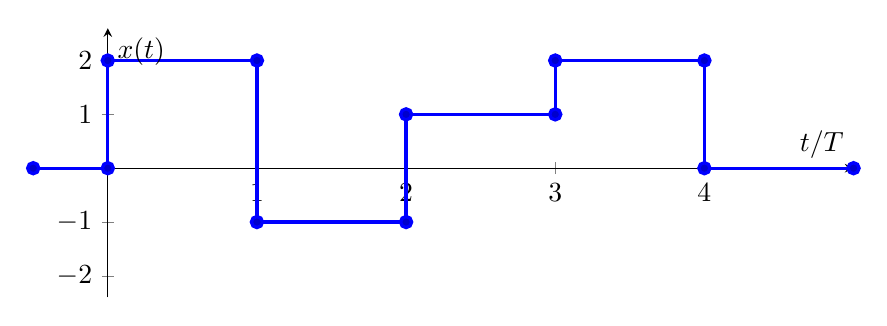
\begin{tikzpicture}
\begin{axis}[
  width=12cm, height=5cm,
  xmin=-0.5, xmax=5, ymin=-2.4, ymax=2.6,
  axis lines=center, xlabel={$t/T$}, ylabel={$x(t)$},
  xtick={1,2,3,4}, ytick={-2,-1,1,2},
  every axis plot/.append style={very thick, blue},
]
\addplot coordinates {(-0.5,0) (0,0) (0,2) (1,2) (1,-1) (2,-1) (2,1) (3,1) (3,2) (4,2) (4,0) (5,0)};
\end{axis}
\end{tikzpicture}
\end{center}

\subsubsection*{a) Darstellung als Summe von Sprungfunktionen}

\begin{beispiel}[Zerlegung in Sprungfunktionen]

\textbf{Gegeben:} Die obige Treppenfunktion.

\textbf{Gesucht:} Darstellung als Summe gewichteter, verschobener
Sprungfunktionen.

\textbf{Formel} (Sprungfunktion, Abschnitt~\ref{sec:elementare-analoge-signale}):
An jeder Sprungstelle $t_i$ wird ein Term $(\Delta x_i)\,\epsilon(t - t_i)$
addiert, wobei $\Delta x_i$ die Sprunghöhe ist.

\textbf{Rechnung:} Die Sprunghöhen betragen

$$
\begin{aligned}
&t=0:\; 0 \to 2 \;(+2), \quad
 t=T:\; 2 \to -1 \;(-3), \quad
 t=2T:\; -1 \to 1 \;(+2), \\
&t=3T:\; 1 \to 2 \;(+1), \quad
 t=4T:\; 2 \to 0 \;(-2).
\end{aligned}
$$

Probe: $2 - 3 + 2 + 1 - 2 = 0$ \checkmark (das Signal endet bei $0$).

\textbf{Lösung:}

$$
\boxed{\;x(t) = 2\,\epsilon(t) - 3\,\epsilon(t-T) + 2\,\epsilon(t-2T)
+ \epsilon(t-3T) - 2\,\epsilon(t-4T).\;}
$$

\end{beispiel}

\subsubsection*{b) Darstellung als Summe von Rechteckfunktionen}

\begin{beispiel}[Zerlegung in Rechteckfunktionen]

\textbf{Gegeben:} Dieselbe Treppenfunktion.

\textbf{Gesucht:} Darstellung als Summe gewichteter Rechteckfunktionen.

\textbf{Formel:} Jeder konstante Abschnitt $[kT,(k+1)T)$ der Höhe $h_k$ wird
durch $h_k \operatorname{rect}\!\left(\dfrac{t-kT}{T}\right)$ dargestellt.

\textbf{Rechnung:} Die vier nichtverschwindenden Stufen besitzen die Höhen
$2,\, -1,\, 1,\, 2$.

\textbf{Lösung:}

$$
\boxed{\;x(t) = 2\operatorname{rect}\!\left(\frac{t}{T}\right)
- \operatorname{rect}\!\left(\frac{t-T}{T}\right)
+ \operatorname{rect}\!\left(\frac{t-2T}{T}\right)
+ 2\operatorname{rect}\!\left(\frac{t-3T}{T}\right).\;}
$$

\end{beispiel}

% ================================================================
\subsection*{Aufgabe 1.3 – Exponentialfunktion}
% ================================================================

Die Funktionen sind für $T = 1\,\mathrm{ms}$ als Funktion von $t$ und $t/T$ zu
zeichnen; abschließend erfolgt die Klassifikation.

\subsubsection*{a) $x(t) = -e^{-t/2T}\,\epsilon(t)$}

\begin{beispiel}[Negative abklingende Exponentialfunktion]

\textbf{Gegeben:} $x(t) = -e^{-t/2T}\,\epsilon(t)$, $T = 1\,\mathrm{ms}$.

\textbf{Gesucht:} Signalverlauf; Energie- oder Leistungssignal?

\textbf{Rechnung:} Für $t \geq 0$ steigt $x(t)$ von $x(0) = -1$ monoton gegen
$0$ (von unten); Zeitkonstante $2T$. Die Energie ist endlich:

$$
E_x = \int_0^{\infty} \left(-e^{-t/2T}\right)^2 \mathrm{d}t
    = \int_0^{\infty} e^{-t/T}\,\mathrm{d}t = T = 1\,\mathrm{ms}.
$$

\begin{center}
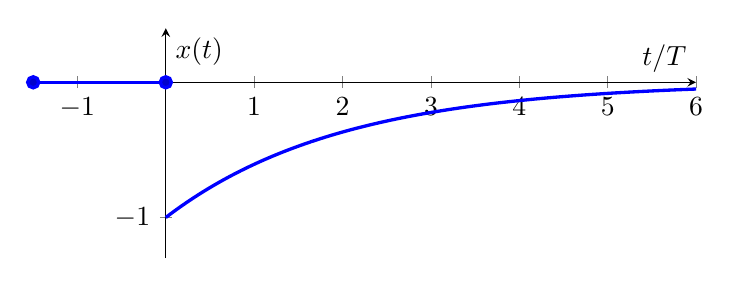
\begin{tikzpicture}
\begin{axis}[
  width=10cm, height=4.5cm,
  xmin=-1.5, xmax=6, ymin=-1.3, ymax=0.4,
  axis lines=center, xlabel={$t/T$}, ylabel={$x(t)$},
  ytick={-1}, yticklabels={$-1$},
  samples=100,
  every axis plot/.append style={very thick, blue},
]
\addplot coordinates {(-1.5,0) (0,0)};
\addplot[domain=0:6] {-exp(-x/2)};
\end{axis}
\end{tikzpicture}
\end{center}

\textbf{Lösung:} $\boxed{\;E_x = T \Rightarrow \text{Energiesignal.}\;}$

\end{beispiel}

\subsubsection*{b) $x(t) = 4\left(1 - \exp\!\left(-\frac{t-2T}{T}\right)\right)\epsilon(t-2T)$}

\begin{beispiel}[Verzögert aufladende Exponentialfunktion]

\textbf{Gegeben:} $x(t) = 4\left(1 - \exp\!\left(-\frac{t-2T}{T}\right)\right)
\epsilon(t-2T)$, $T = 1\,\mathrm{ms}$.

\textbf{Gesucht:} Signalverlauf; Energie- oder Leistungssignal?

\textbf{Rechnung:} Für $t \geq 2T$ steigt $x(t)$ von $0$ monoton gegen den
Grenzwert $4$ (Zeitkonstante $T$). Da $x(t) \to 4$ konstant bleibt, ist
$E_x = \infty$ und

$$
P_x = \lim_{T_0 \to \infty} \frac{1}{2T_0}\int_{2T}^{T_0}
      16\left(1 - e^{-(t-2T)/T}\right)^2 \mathrm{d}t = \frac{16}{2} = 8.
$$

\begin{center}
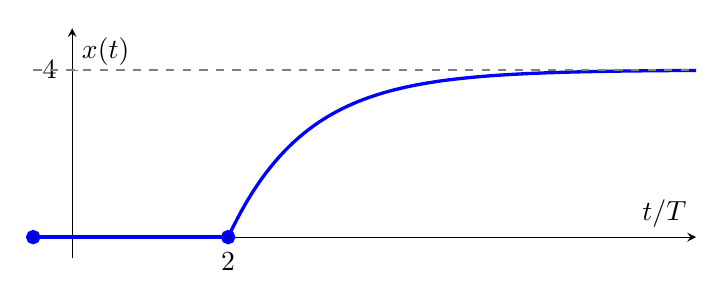
\begin{tikzpicture}
\begin{axis}[
  width=10cm, height=4.5cm,
  xmin=-0.5, xmax=8, ymin=-0.5, ymax=5,
  axis lines=center, xlabel={$t/T$}, ylabel={$x(t)$},
  xtick={2}, ytick={4}, yticklabels={$4$},
  samples=100,
  every axis plot/.append style={very thick, blue},
]
\addplot coordinates {(-0.5,0) (2,0)};
\addplot[domain=2:8] {4*(1-exp(-(x-2)))};
\draw[dashed, gray] (axis cs:-0.5,4) -- (axis cs:8,4);
\end{axis}
\end{tikzpicture}
\end{center}

\textbf{Lösung:} $\boxed{\;P_x = 8 \Rightarrow \text{Leistungssignal.}\;}$

\end{beispiel}

% ================================================================
\subsection*{Aufgabe 1.4 – Harmonische Zeitfunktionen}
% ================================================================

Für jedes Signal sind Periodendauer $T$, Frequenz $f = 1/T$, Kreisfrequenz
$\omega = 2\pi/T$, Mittelwert, Leistung und Symmetrieeigenschaft zu bestimmen.
Für die Leistung periodischer Signale gilt
$P_x = \frac{1}{T}\int_0^T |x(t)|^2\,\mathrm{d}t$
(Abschnitt~\ref{sec:leistung}); die Leistung einer harmonischen Schwingung der
Amplitude $A$ beträgt $A^2/2$.

\subsubsection*{a) $x(t) = -\sin\!\left(\frac{2\pi}{4\,\mathrm{s}}t + \frac{\pi}{2}\right)$}

\begin{beispiel}[Phasenverschobene Sinusschwingung]

\textbf{Gegeben:} $x(t) = -\sin\!\left(\dfrac{2\pi}{4\,\mathrm{s}}t + \dfrac{\pi}{2}\right)$.

\textbf{Gesucht:} $T,\, f,\, \omega$, Mittelwert, Leistung, Symmetrie.

\textbf{Rechnung:} Mit $\sin(\theta + \tfrac{\pi}{2}) = \cos\theta$ folgt
$x(t) = -\cos\!\left(\dfrac{\pi}{2}\,t\right)$. Damit

$$
\omega = \frac{\pi}{2}\,\mathrm{s}^{-1}, \qquad
T = \frac{2\pi}{\omega} = 4\,\mathrm{s}, \qquad
f = \frac{1}{T} = \frac{1}{4}\,\mathrm{Hz}.
$$

Da $-\cos$ gerade ist, ist $x(t)$ \emph{gerade}. Mittelwert $\bar{x} = 0$,
Leistung $P_x = \dfrac{1^2}{2} = \dfrac{1}{2}$.

\begin{center}
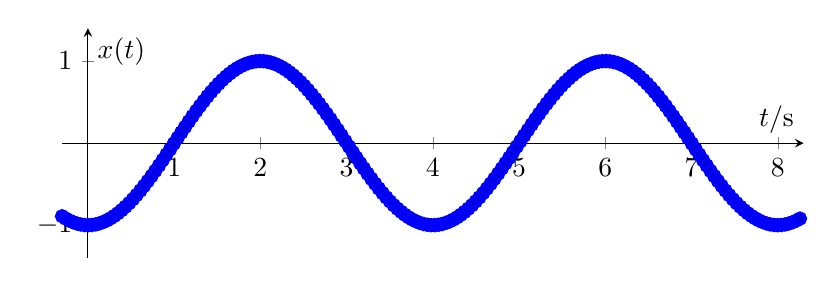
\begin{tikzpicture}
\begin{axis}[
  width=11cm, height=4.5cm,
  xmin=-0.3, xmax=8.3, ymin=-1.4, ymax=1.4,
  axis lines=center, xlabel={$t/\mathrm{s}$}, ylabel={$x(t)$},
  ytick={-1,1}, samples=200, domain=-0.3:8.3,
  every axis plot/.append style={very thick, blue},
]
\addplot {-cos(90*x)};
\end{axis}
\end{tikzpicture}
\end{center}

\textbf{Lösung:}
$\boxed{\;T = 4\,\mathrm{s},\; f = \tfrac14\,\mathrm{Hz},\;
\omega = \tfrac{\pi}{2}\,\mathrm{s}^{-1};\; \text{gerade},\;
\bar{x} = 0,\; P_x = \tfrac12.\;}$

\end{beispiel}

\subsubsection*{b) $x(t) = 1 + \cos\!\left(\frac{\pi t}{1\,\mathrm{s}} + \pi\right)$}

\begin{beispiel}[Kosinusschwingung mit Gleichanteil]

\textbf{Gegeben:} $x(t) = 1 + \cos\!\left(\dfrac{\pi t}{1\,\mathrm{s}} + \pi\right)$.

\textbf{Gesucht:} $T,\, f,\, \omega$, Mittelwert, Leistung, Symmetrie.

\textbf{Rechnung:} Mit $\cos(\theta + \pi) = -\cos\theta$ folgt
$x(t) = 1 - \cos(\pi t)$. Damit

$$
\omega = \pi\,\mathrm{s}^{-1}, \qquad T = 2\,\mathrm{s}, \qquad
f = \tfrac12\,\mathrm{Hz}.
$$

$x(t)$ ist \emph{gerade}. Der Gleichanteil liefert den Mittelwert
$\bar{x} = 1$. Die Leistung setzt sich aus Gleich- und Wechselanteil zusammen:

$$
P_x = \frac{1}{T}\int_0^T (1 - \cos\pi t)^2\,\mathrm{d}t
    = 1^2 + \frac{1^2}{2} = \frac{3}{2}.
$$

\begin{center}
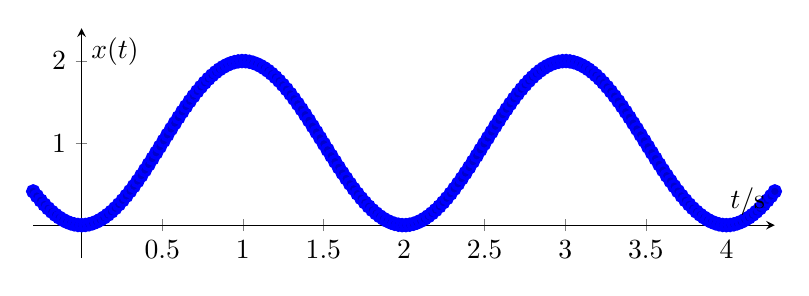
\begin{tikzpicture}
\begin{axis}[
  width=11cm, height=4.5cm,
  xmin=-0.3, xmax=4.3, ymin=-0.4, ymax=2.4,
  axis lines=center, xlabel={$t/\mathrm{s}$}, ylabel={$x(t)$},
  ytick={1,2}, samples=200, domain=-0.3:4.3,
  every axis plot/.append style={very thick, blue},
]
\addplot {1-cos(180*x)};
\end{axis}
\end{tikzpicture}
\end{center}

\textbf{Lösung:}
$\boxed{\;T = 2\,\mathrm{s},\; f = \tfrac12\,\mathrm{Hz},\;
\omega = \pi\,\mathrm{s}^{-1};\; \text{gerade},\;
\bar{x} = 1,\; P_x = \tfrac32.\;}$

\end{beispiel}

\subsubsection*{c) $x(t) = \cos\!\left(\frac{100\pi}{1\,\mathrm{s}}t\right)$}

\begin{beispiel}[Hochfrequente Kosinusschwingung]

\textbf{Gegeben:} $x(t) = \cos\!\left(\dfrac{100\pi}{1\,\mathrm{s}}\,t\right)$.

\textbf{Gesucht:} $T,\, f,\, \omega$, Mittelwert, Leistung, Symmetrie.

\textbf{Rechnung:}

$$
\omega = 100\pi\,\mathrm{s}^{-1}, \qquad
T = \frac{2\pi}{\omega} = \frac{1}{50}\,\mathrm{s} = 20\,\mathrm{ms}, \qquad
f = 50\,\mathrm{Hz}.
$$

$x(t)$ ist \emph{gerade}, $\bar{x} = 0$, $P_x = \dfrac{1^2}{2} = \dfrac{1}{2}$.

\begin{center}
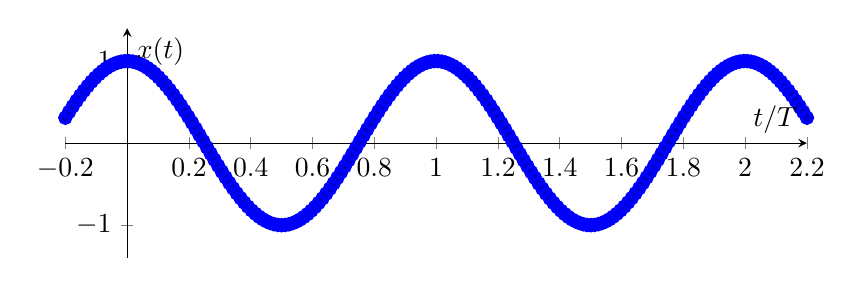
\begin{tikzpicture}
\begin{axis}[
  width=11cm, height=4.5cm,
  xmin=-0.2, xmax=2.2, ymin=-1.4, ymax=1.4,
  axis lines=center, xlabel={$t/T$}, ylabel={$x(t)$},
  ytick={-1,1}, samples=200, domain=-0.2:2.2,
  every axis plot/.append style={very thick, blue},
]
\addplot {cos(360*x)};
\end{axis}
\end{tikzpicture}
\end{center}

\textbf{Lösung:}
$\boxed{\;T = 20\,\mathrm{ms},\; f = 50\,\mathrm{Hz},\;
\omega = 100\pi\,\mathrm{s}^{-1};\; \text{gerade},\;
\bar{x} = 0,\; P_x = \tfrac12.\;}$

\end{beispiel}

% ================================================================
\subsection*{Aufgabe 1.5 – Zusammenfassung zweier Harmonischer}
% ================================================================

\begin{beispiel}[Amplitude und Phase der Summe zweier Harmonischer]

\textbf{Gegeben:} $x(t) = \sin(\omega t) + \cos(\omega t)$.

\textbf{Gesucht:} Amplitude $A$ und Phase $\varphi$ so, dass
$x(t) = A\sin(\omega t + \varphi)$.

\textbf{Formel} (Additionstheorem):

$$
A\sin(\omega t + \varphi) = A\cos\varphi\,\sin(\omega t)
+ A\sin\varphi\,\cos(\omega t).
$$

\textbf{Rechnung:} Koeffizientenvergleich mit
$\sin(\omega t) + \cos(\omega t)$:

$$
A\cos\varphi = 1, \qquad A\sin\varphi = 1.
$$

Quadrieren und Addieren liefert $A^2(\cos^2\varphi + \sin^2\varphi) = 2$, also
$A = \sqrt{2}$. Der Quotient ergibt $\tan\varphi = 1$, und da beide
Komponenten positiv sind, liegt $\varphi$ im ersten Quadranten:
$\varphi = \dfrac{\pi}{4}$.

\textbf{Lösung:}

$$
\boxed{\;x(t) = \sqrt{2}\,\sin\!\left(\omega t + \frac{\pi}{4}\right).\;}
$$

\end{beispiel}

% ================================================================
\subsection*{Aufgabe 1.6 – Signaleigenschaften}
% ================================================================

Zu bestimmen sind Periodizität, Symmetrie, der Mittelwert im Zeitintervall mit
$x(t) \neq 0$ sowie die Klassifikation als Energie- oder Leistungssignal (mit
Energie- bzw.\ Leistungswert).

\subsubsection*{a) $x(t) = \sin(\omega t)$, $\omega = 2\pi\frac{1}{T}$}

\begin{beispiel}[Reine Sinusschwingung]

\textbf{Gegeben:} $x(t) = \sin(\omega t)$ mit $\omega = 2\pi/T$.

\textbf{Gesucht:} Periodizität, Symmetrie, Mittelwert, Klassifikation.

\textbf{Rechnung:} $x(t)$ ist \emph{periodisch} mit Periode $T$ und
\emph{ungerade}. Über eine Periode ist $\bar{x} = 0$. Als periodisches Signal
mit $E_x = \infty$ liegt ein Leistungssignal vor:

$$
P_x = \frac{1}{T}\int_0^T \sin^2(\omega t)\,\mathrm{d}t = \frac{1}{2}.
$$

\textbf{Lösung:}
$\boxed{\;\text{periodisch, ungerade},\; \bar{x} = 0,\;
P_x = \tfrac12 \Rightarrow \text{Leistungssignal.}\;}$

\end{beispiel}

\subsubsection*{b) $x(t) = \operatorname{rect}\!\left(\frac{t}{2T}\right)\cdot\frac{t}{2T}$}

\begin{beispiel}[Einseitige Rampe]

\textbf{Gegeben:} $x(t) = \operatorname{rect}\!\left(\dfrac{t}{2T}\right)
\cdot \dfrac{t}{2T}$.

\textbf{Gesucht:} Periodizität, Symmetrie, Mittelwert, Klassifikation.

\textbf{Rechnung:} Die Rechteckfunktion ist $1$ für $0 \leq t < 2T$; dort ist
$x(t) = \dfrac{t}{2T}$, also eine Rampe von $0$ auf $1$. Sonst $0$. Das Signal
ist \emph{nicht periodisch} und weist \emph{keine} Symmetrie auf. Mittelwert
über den Träger $[0, 2T)$:

$$
\bar{x} = \frac{1}{2T}\int_0^{2T} \frac{t}{2T}\,\mathrm{d}t
        = \frac{1}{2T}\cdot\frac{1}{2T}\cdot\frac{(2T)^2}{2} = \frac{1}{2}.
$$

Endliche Dauer, also Energiesignal:

$$
E_x = \int_0^{2T} \left(\frac{t}{2T}\right)^2 \mathrm{d}t
    = \frac{1}{4T^2}\cdot\frac{(2T)^3}{3} = \frac{2T}{3}.
$$

\begin{center}
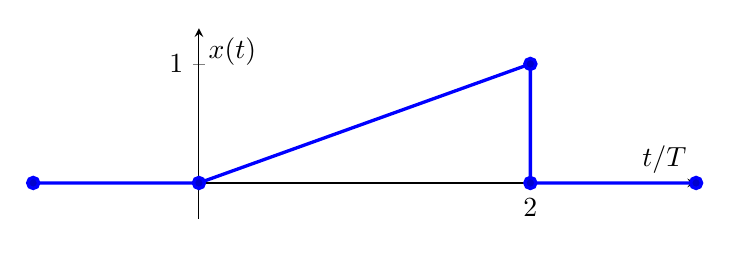
\begin{tikzpicture}
\begin{axis}[
  width=10cm, height=4cm,
  xmin=-1, xmax=3, ymin=-0.3, ymax=1.3,
  axis lines=center, xlabel={$t/T$}, ylabel={$x(t)$},
  xtick={2}, ytick={1}, yticklabels={$1$},
  every axis plot/.append style={very thick, blue},
]
\addplot coordinates {(-1,0) (0,0) (2,1) (2,0) (3,0)};
\end{axis}
\end{tikzpicture}
\end{center}

\textbf{Lösung:}
$\boxed{\;\text{nicht periodisch, keine Symmetrie},\; \bar{x} = \tfrac12,\;
E_x = \tfrac{2T}{3} \Rightarrow \text{Energiesignal.}\;}$

\end{beispiel}

\subsubsection*{c) $x(t) = \left[\epsilon(t+T) - \epsilon(t-T)\right]\frac{|t|}{T}$}

\begin{beispiel}[Symmetrisches Dreiecksignal]

\textbf{Gegeben:} $x(t) = \left[\epsilon(t+T) - \epsilon(t-T)\right]\dfrac{|t|}{T}$.

\textbf{Gesucht:} Periodizität, Symmetrie, Mittelwert, Klassifikation.

\textbf{Rechnung:} Die Klammer ist $1$ für $-T \leq t < T$; dort ist
$x(t) = \dfrac{|t|}{T}$ (V-Form, $0$ bei $t = 0$, $1$ bei $t = \pm T$). Das
Signal ist \emph{nicht periodisch}, aber \emph{gerade} (wegen $|t|$).
Mittelwert über $[-T, T)$:

$$
\bar{x} = \frac{1}{2T}\int_{-T}^{T} \frac{|t|}{T}\,\mathrm{d}t
        = \frac{1}{2T}\cdot\frac{2}{T}\cdot\frac{T^2}{2} = \frac{1}{2}.
$$

Energiesignal mit

$$
E_x = \int_{-T}^{T} \frac{t^2}{T^2}\,\mathrm{d}t
    = \frac{2}{T^2}\cdot\frac{T^3}{3} = \frac{2T}{3}.
$$

\begin{center}
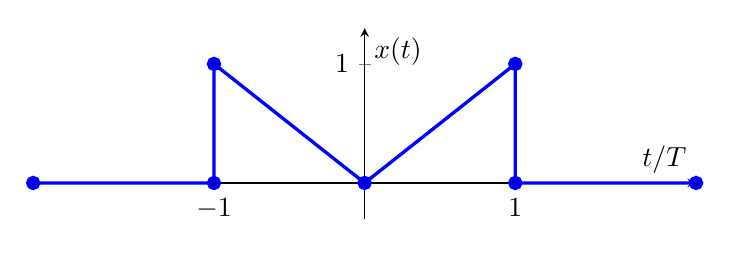
\begin{tikzpicture}
\begin{axis}[
  width=10cm, height=4cm,
  xmin=-2.2, xmax=2.2, ymin=-0.3, ymax=1.3,
  axis lines=center, xlabel={$t/T$}, ylabel={$x(t)$},
  xtick={-1,1}, ytick={1}, yticklabels={$1$},
  every axis plot/.append style={very thick, blue},
]
\addplot coordinates {(-2.2,0) (-1,0) (-1,1) (0,0) (1,1) (1,0) (2.2,0)};
\end{axis}
\end{tikzpicture}
\end{center}

\textbf{Lösung:}
$\boxed{\;\text{nicht periodisch, gerade},\; \bar{x} = \tfrac12,\;
E_x = \tfrac{2T}{3} \Rightarrow \text{Energiesignal.}\;}$

\end{beispiel}

\subsubsection*{d) $x(t) = \operatorname{si}\!\left(\frac{t}{T}\right)$}

\begin{beispiel}[Spaltfunktion (si-Funktion)]

\textbf{Gegeben:} $x(t) = \operatorname{si}\!\left(\dfrac{t}{T}\right)
= \dfrac{\sin(t/T)}{t/T}$.

\textbf{Gesucht:} Periodizität, Symmetrie, Mittelwert, Klassifikation.

\textbf{Rechnung:} Die si-Funktion ist \emph{nicht periodisch} (nur ihre
Nullstellen liegen periodisch) und \emph{gerade}. Sie klingt für
$|t| \to \infty$ ab; ihr zeitlicher Mittelwert verschwindet:
$\bar{x} = 0$. Mit der Substitution $u = t/T$ und
$\int_{-\infty}^{\infty}\frac{\sin^2 u}{u^2}\,\mathrm{d}u = \pi$ folgt die
endliche Energie:

$$
E_x = \int_{-\infty}^{\infty} \operatorname{si}^2\!\left(\frac{t}{T}\right)
      \mathrm{d}t
    = T\int_{-\infty}^{\infty} \frac{\sin^2 u}{u^2}\,\mathrm{d}u
    = \pi T.
$$

\begin{center}
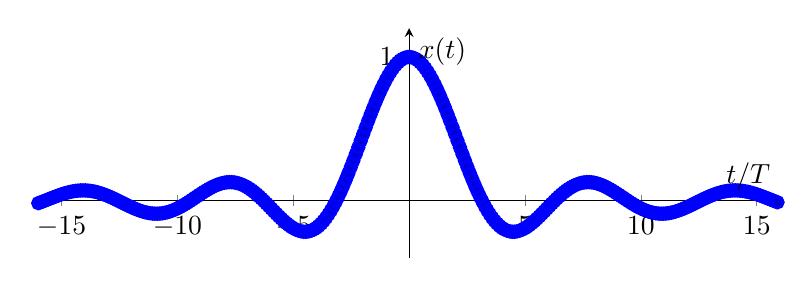
\begin{tikzpicture}
\begin{axis}[
  width=11cm, height=4.5cm,
  xmin=-16, xmax=16, ymin=-0.4, ymax=1.2,
  axis lines=center, xlabel={$t/T$}, ylabel={$x(t)$},
  ytick={1}, yticklabels={$1$},
  samples=300, domain=-16:16,
  every axis plot/.append style={very thick, blue},
]
\addplot {sin(deg(x))/x};
\end{axis}
\end{tikzpicture}
\end{center}

\textbf{Lösung:}
$\boxed{\;\text{nicht periodisch, gerade},\; \bar{x} = 0,\;
E_x = \pi T \Rightarrow \text{Energiesignal.}\;}$

\end{beispiel}

% ================================================================
\subsection*{Aufgabe 1.7 – Komplexwertige Signale}
% ================================================================

Für die folgenden komplexwertigen Signale
(Abschnitt~\ref{sec:komplexwertige-signale}) sind Real- und Imaginärteil,
Periodendauer $T$, Frequenz $f$, Mittelwert und Leistung zu bestimmen. Für ein
komplexwertiges periodisches Signal gilt

$$
\bar{\underline{x}} = \frac{1}{T}\int_0^T \underline{x}(t)\,\mathrm{d}t,
\qquad
P_{\underline{x}} = \frac{1}{T}\int_0^T |\underline{x}(t)|^2\,\mathrm{d}t.
$$

Wegen $|\underline{x}|^2 = \operatorname{Re}\{\underline{x}\}^2
+ \operatorname{Im}\{\underline{x}\}^2$ und
$\underline{x} = \operatorname{Re}\{\underline{x}\}
+ j\operatorname{Im}\{\underline{x}\}$ gilt für die Mittelwerte und Leistungen
stets

$$
\bar{\underline{x}} = \overline{\operatorname{Re}\{\underline{x}\}}
+ j\,\overline{\operatorname{Im}\{\underline{x}\}},
\qquad
P_{\underline{x}} = P_{\operatorname{Re}\{\underline{x}\}}
+ P_{\operatorname{Im}\{\underline{x}\}}.
$$

\subsubsection*{a) $\underline{x}(t) = \sqrt{2}\,e^{j\left(\frac{2\pi t}{2\,\mathrm{ms}} - \frac{\pi}{2}\right)}$}

\begin{beispiel}[Komplexes Exponentialsignal mit konstantem Betrag]

\textbf{Gegeben:}
$\underline{x}(t) = \sqrt{2}\,e^{j\left(\frac{2\pi t}{2\,\mathrm{ms}}
- \frac{\pi}{2}\right)}$.

\textbf{Gesucht:} $\operatorname{Re}$, $\operatorname{Im}$, $T$, $f$,
Mittelwert, Leistung.

\textbf{Rechnung:} Aus $\omega = \dfrac{2\pi}{2\,\mathrm{ms}}
= \dfrac{\pi}{1\,\mathrm{ms}}$ folgt $T = 2\,\mathrm{ms}$, $f = 500\,\mathrm{Hz}$.
Mit $\cos(\omega t - \tfrac{\pi}{2}) = \sin(\omega t)$ und
$\sin(\omega t - \tfrac{\pi}{2}) = -\cos(\omega t)$:

$$
\operatorname{Re}\{\underline{x}(t)\} = \sqrt{2}\,\sin(\omega t),
\qquad
\operatorname{Im}\{\underline{x}(t)\} = -\sqrt{2}\,\cos(\omega t).
$$

Der Betrag $|\underline{x}| = \sqrt{2}$ ist konstant, das Signal rotiert einmal
pro Periode:

$$
\bar{\underline{x}} = 0, \qquad
P_{\underline{x}} = |\underline{x}|^2 = 2.
$$

Kontrolle über Real- und Imaginärteil: beide sind Sinusgrößen der Amplitude
$\sqrt{2}$, also
$P_{\operatorname{Re}} = P_{\operatorname{Im}} = \dfrac{(\sqrt{2})^2}{2} = 1$
und $\overline{\operatorname{Re}} = \overline{\operatorname{Im}} = 0$; damit
$P_{\underline{x}} = 1 + 1 = 2$ \checkmark.

\textbf{Lösung:}

$$
\boxed{\;\operatorname{Re} = \sqrt{2}\sin(\omega t),\;
\operatorname{Im} = -\sqrt{2}\cos(\omega t);\;
T = 2\,\mathrm{ms},\; f = 500\,\mathrm{Hz},\;
\bar{\underline{x}} = 0,\; P_{\underline{x}} = 2.\;}
$$

\end{beispiel}

\subsubsection*{b) $\underline{x}(t) = j + 2e^{j\left(\frac{2\pi t}{4\,\mathrm{ms}} + \frac{\pi}{4}\right)}$}

\begin{beispiel}[Komplexes Exponentialsignal mit Gleichanteil]

\textbf{Gegeben:}
$\underline{x}(t) = j + 2e^{j\left(\frac{2\pi t}{4\,\mathrm{ms}}
+ \frac{\pi}{4}\right)}$.

\textbf{Gesucht:} $\operatorname{Re}$, $\operatorname{Im}$, $T$, $f$,
Mittelwert, Leistung.

\textbf{Rechnung:} Aus $\omega = \dfrac{2\pi}{4\,\mathrm{ms}}
= \dfrac{\pi}{2\,\mathrm{ms}}$ folgt $T = 4\,\mathrm{ms}$, $f = 250\,\mathrm{Hz}$.
Mit $\theta = \omega t + \tfrac{\pi}{4}$:

$$
\operatorname{Re}\{\underline{x}(t)\} = 2\cos\theta,
\qquad
\operatorname{Im}\{\underline{x}(t)\} = 1 + 2\sin\theta.
$$

Der rotierende Term mittelt sich zu $0$, der konstante Anteil $j$ bleibt:

$$
\bar{\underline{x}} = j.
$$

Für die Leistung mit $|\underline{x}|^2 = (2\cos\theta)^2
+ (1 + 2\sin\theta)^2 = 5 + 4\sin\theta$:

$$
P_{\underline{x}} = \frac{1}{T}\int_0^T (5 + 4\sin\theta)\,\mathrm{d}t = 5
= \underbrace{|j|^2}_{1} + \underbrace{|2|^2}_{4}.
$$

Kontrolle: $P_{\operatorname{Re}} = \overline{4\cos^2\theta} = 2$,
$P_{\operatorname{Im}} = \overline{(1 + 2\sin\theta)^2} = 1 + 2 = 3$; Summe
$= 5$ \checkmark. Ferner $\overline{\operatorname{Re}} = 0$,
$\overline{\operatorname{Im}} = 1$.

\textbf{Lösung:}

$$
\boxed{\;\operatorname{Re} = 2\cos\theta,\;
\operatorname{Im} = 1 + 2\sin\theta,\;\theta = \omega t + \tfrac{\pi}{4};\;
T = 4\,\mathrm{ms},\; f = 250\,\mathrm{Hz},\;
\bar{\underline{x}} = j,\; P_{\underline{x}} = 5.\;}
$$

\end{beispiel}

\subsubsection*{c) $\underline{x}(t) = 5 - j + 3\exp\!\left(\frac{j2\pi t}{10\,\mathrm{ms}}\right)$}

\begin{beispiel}[Komplexes Exponentialsignal mit komplexem Gleichanteil]

\textbf{Gegeben:}
$\underline{x}(t) = 5 - j + 3\exp\!\left(\dfrac{j2\pi t}{10\,\mathrm{ms}}\right)$.

\textbf{Gesucht:} $\operatorname{Re}$, $\operatorname{Im}$, $T$, $f$,
Mittelwert, Leistung.

\textbf{Rechnung:} Aus $\omega = \dfrac{2\pi}{10\,\mathrm{ms}}$ folgt
$T = 10\,\mathrm{ms}$, $f = 100\,\mathrm{Hz}$. Mit
$3e^{j\omega t} = 3\cos\omega t + j\,3\sin\omega t$:

$$
\operatorname{Re}\{\underline{x}(t)\} = 5 + 3\cos\omega t,
\qquad
\operatorname{Im}\{\underline{x}(t)\} = -1 + 3\sin\omega t.
$$

Der rotierende Term mittelt sich zu $0$:

$$
\bar{\underline{x}} = 5 - j.
$$

Leistung (Gleichanteil plus rotierender Term):

$$
P_{\underline{x}} = |5 - j|^2 + |3|^2 = (25 + 1) + 9 = 35.
$$

Kontrolle: $P_{\operatorname{Re}} = \overline{(5 + 3\cos\omega t)^2}
= 25 + \tfrac{9}{2} = 29{,}5$ und
$P_{\operatorname{Im}} = \overline{(-1 + 3\sin\omega t)^2}
= 1 + \tfrac{9}{2} = 5{,}5$; Summe $= 35$ \checkmark. Ferner
$\overline{\operatorname{Re}} = 5$, $\overline{\operatorname{Im}} = -1$.

\textbf{Lösung:}

$$
\boxed{\;\operatorname{Re} = 5 + 3\cos\omega t,\;
\operatorname{Im} = -1 + 3\sin\omega t;\;
T = 10\,\mathrm{ms},\; f = 100\,\mathrm{Hz},\;
\bar{\underline{x}} = 5 - j,\; P_{\underline{x}} = 35.\;}
$$

Der Mittelwert des komplexen Signals ist stets die Summe der Mittelwerte von
Real- und Imaginärteil (letzterer mit $j$ gewichtet), die Gesamtleistung die
Summe der Leistungen von Real- und Imaginärteil.

\end{beispiel}
